\chapter{聴覚と音声信号}
\section{\kadaida}\label{sec:\kadaida}
\purpose
\paragraph{音脈分凝とは}
例として,音列\ \fbox{C4\ G4\ C4\ G4\ C4\ G4\ \dots}\ をあげる.この音列を長く聴いた場合,テンポが遅いと音列は「旋律」として聞こえるが,テンポを早くするについれて\ \fbox{C4\ C4\ C4\ \dots} \ \fbox{G4\ G4\ G4\ \dots}と,音列が分離して聞こえる.
この現象を音脈分凝と呼ぶ.また,テンポを一定にした場合,2つの音程差(C4とG4は完全5度)が大きいほど,音脈分凝が生じやすい.\cite[p.182]{感覚知覚心理学}
\paragraph{実験}
今回の実験では,テンポを一定にした場合の,周波数による音脈分凝の生じ方について調査する.
音脈分凝が生じる波形を作成し,音脈分凝が生じる周波数組み合わせと,音脈分凝が生じにくい組み合わせを実験により発見する.
\method
サンプリング周波数を\(16\textrm{kHz}\),1音を\(0.2\)秒に設定し,音Aと音Bを連結させた音Cを10回繰り返す.
正弦波の行列を連結するために,\texttt{repmat}関数を用いる.実験する周波数の組み合わせを\tblref{tbl:音脈分凝_実験結果}に示す.周波数\(f_A\)と周波数\(f_B\)の差を\(f_D=\big|f_A-f_B\big|\)と定義する.
\scall\sref{src:04_01}.
\result
聴音確認による結果を\tblref{tbl:音脈分凝_実験結果}に示す.
\begin{table}[h]
    \centering
    \caption{音脈分凝\ 実験結果}
    \label{tbl:音脈分凝_実験結果}
    \begin{tabularx}{\textwidth}{ccccR}
            & 周波数\(f_A\) & 周波数\(f_B\) & 周波数差\(f_D\) & \multicolumn{1}{c}{実験結果}                                    \\
        \hline
        実験1 & \(1000\)   & \(990\)    & \(10\)      & 音脈分凝は生じず,滑らかな音に聞こえた.                                        \\
        実験2 & \(1000\)   & \(800\)    & \(200\)     & 音脈分凝は生じず,別音の組み合わせによる旋律に聞こえた.                                \\
        実験3 & \(1000\)   & \(200\)    & \(800\)     & 音脈分凝が生じ,\(1000\textrm{Hz}\),\(200\textrm{Hz}\)の2音が分離して聞こえた. \\
        \hline
    \end{tabularx}
\end{table}
\consideration
結果より,周波数組み合わせの差\(f_D\)が大きいほど音脈分凝が生じやすいこと,\(f_D=10\)程度であれば音の切れ目すら聞こえないことが分かった.
今回の実験では,3つの組み合わせのみ実験したため,音脈分凝が生じる具体的な周波数差\(f_D\)は分からなかった.テンポによる音脈分凝の生じやすさについても,今後の課題として調査したい.
\section{\kadaidb}\label{sec:\kadaidb}
\purpose
\paragraph{連続聽効果とは}
ある一連の音を一部,短時間だけ削除し,雑音に置き換える.
ヒトは,「もとの音声の中に雑音が混入された」と知覚し,部分的な削除には気付かない.この現象を聴覚的補完,または連続聴効果と呼ぶ.\cite[p.182\ -\ p.183]{感覚知覚心理学}
\paragraph{実験}
連続聴効果が生じやすい刺激と,連続聴効果が生じにくい刺激を作成する.雑音や純音の周波数と,連続聴効果の関係について明らかにする.
\method
\paragraph{雑音の作成}
雑音を,白色雑音(ノイズA)と白色雑音からフィルタ処理により,周波数の\(1020\textrm{Hz}\)から\(1620\textrm{Hz}\)を除去した雑音(ノイズB)を作成する.
白色雑音は,振幅\(1\),サンプリング周波数\(16\texttt{kHz}\)で構成する.白色雑音は,周波数成分を均等に含むパワースペクトルが一定である,不規則な波である.(\ref{sec:\kadaiae}章)
ゆえに,乱数を\texttt{rand}関数を用いて生成し,白色雑音を作成する.
\texttt{rand}関数は,\(0\)から\(1\)までの実数を戻り値としているため,\texttt{rand}関数で\(-1\)から\(1\)までの実数を戻り値としたいときは,各要素から\(-0.5\)し,全データを\(2\)倍する.\par
周波数の\(1020\textrm{Hz}\)から\(1620\textrm{Hz}\)を除去するとき,\texttt{fft}の戻り値を考慮してフィルタを作成する.(\srcref{src:白色雑音の作成})
\figref{fig:ノイズAのFFT後}と\figref{fig:ノイズBのFFT後}を比較すると,ノイズBに周波数フィルタの適用が確認される.
フィルタを通した振幅スペクトルに対して,逆フーリエ変換することで音波を形成する.\par
\paragraph{連続聴効果が生じる音刺激の作成}純音の周波数は,純音A\(=400\textrm{Hz}\),純音B\(=1300\textrm{Hz}\)で作成する.純音BはノイズBに存在しない周波数を設定した.
純音\(1\)秒,雑音\(0.1\)秒を4回繰り返したものを実験する音刺激とする.実験する周波数の組み合わせを\tblref{tbl:連続聴効果}に示す.\scall\sref{src:04_02}.
\begin{lstlisting}[caption={白色雑音の作成},label={src:白色雑音の作成}]
white_noise = 2 * (rand(1,Fs) - 0.5); % 白色雑音の作成
B_fft = fftshift(fft(白色雑音)); % フーリエ変換
noise_filter = ones(1,Fs);
filter_rangeS = 1020; filter_rangeG = 1620; % カット終始 周波数
noise_filter((Fs/2)-filter_rangeG : (Fs/2)-filter_rangeS) = 0; % フィルタの作成
noise_filter((Fs/2)+filter_rangeS : (Fs/2)+filter_rangeG) = 0; % フィルタの作成
B_fft = noise_filter.* A_fft; % 各要素とフィルタの積を取る
noise_B = real(ifft(ifftshift(B_fft))); % 虚部を含むため,real関数を用いる
\end{lstlisting}
\begin{figure}[H]
    \centering
    \begin{minipage}{.45\textwidth}
        \centering
        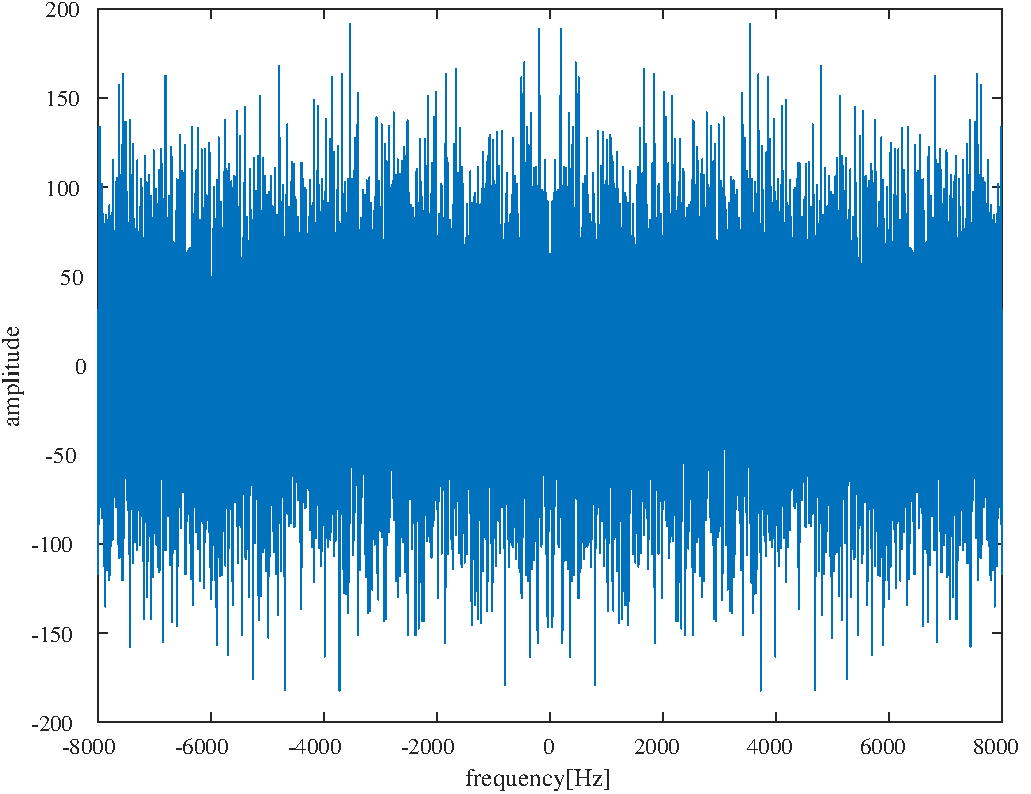
\includegraphics[keepaspectratio,width=\textwidth]{../../Figures/04_20_Afft.pdf}
        \caption{ノイズAの\texttt{fft}後}
        \label{fig:ノイズAのFFT後}
    \end{minipage}
    \hspace{1em}
    \begin{minipage}{.45\textwidth}
        \centering
        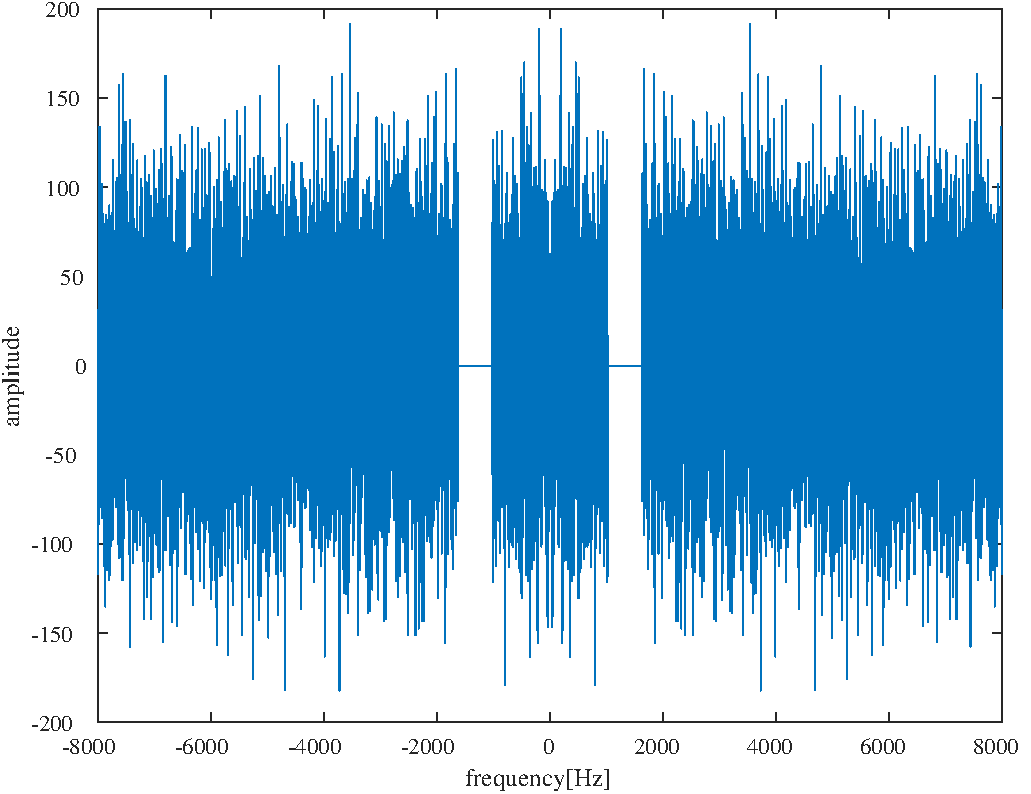
\includegraphics[keepaspectratio,width=\textwidth]{../../Figures/04_21_Bfft.pdf}
        \caption{ノイズBの\texttt{fft}後}
        \label{fig:ノイズBのFFT後}
    \end{minipage}
\end{figure}
\result
実験結果を\tblref{tbl:連続聴効果}に示す.
\begin{table}[h]
    \caption{連続聴効果の実験組み合わせと結果}
    \label{tbl:連続聴効果}
    \begin{tabularx}{\textwidth}{cccR}
            & 純音  & 挿入するノイズ & \multicolumn{1}{c}{実験結果}  \\
        \hline
        実験1 & 純音A & ノイズA    & 雑音部で小さい純音が聞き取れた.          \\
        実験2 & 純音A & ノイズB    & 雑音部で小さい純音が聞き取れた.          \\
        実験3 & 純音B & ノイズA    & 雑音部で小さい純音が聞き取れた.          \\
        実験4 & 純音B & ノイズB    & 雑音部で純音は聞き取れず,純音が非連続に聞こえた. \\
        \hline
    \end{tabularx}
\end{table}
\consideration
実験結果より,純音の周波数がノイズの周波数に含まれていないとき,連続聴効果は生じなかった.
挿入されるノイズに純音の周波数が含まれているとき,雑音の周波数をもとに,脳内で純音を補完していると考えられる.
ゆえに,純音の周波数をノイズから削除すると,連続聴効果が生じにくいと考えられる.\par
今回は純音に対する連続聴効果を実験したが,馴染み深い言語(日本語のフレーズ)に対して雑音を挿入すると,純音に比べて連続聴効果を知覚できるのではないだろうか.日ごろから日本語を聞きなれている我々なら,より強く補完が働くだろう.
\section{\kadaidc}\label{sec:\kadaidc}
\purpose
\paragraph{ミッシングファンダメンタルとは}
人間の聴覚系では,「基本周波数の推定」を行っている.基本周波数成分が物理的に存在しなくても,倍音成分から基本周波数を推定できる.
たとえば,\(300\textrm{Hz}\),\(400\textrm{Hz}\),\(500\textrm{Hz}\)が同時に存在すれば,基本周波数\(100\textrm{Hz}\)を知覚できる\cite{ミッシング・ファンダメンタル_NTTi}.
ミッシングファンダメンタルとは,残っている周波数成分から推定された,基本周波数成分のことである.\par
\paragraph{実験}
今回の実験では,矩形波,ノコギリ波の各波形を加工してミッシングファンダメンタル波を作成する.作成したミッシングファンダメンタル波と原波形を比較して,波形や音の違いについて考察する.
\method
矩形波を例に考える.\ref{sec:\kadaiad}章より,矩形波は\eqref{equ:矩形波}のように三角関数の合成で表すことができる.基本周波数は\(k=1\)で表され,基本周波数の三角関数\(f_1\)は,\eqref{equ:矩形波_基本周波数}である.
\begin{align}
    f_1(t) & =\sin(2\pi ft)\label{equ:矩形波_基本周波数}
\end{align}
今回は,原波形とミッシングファンダメンタル波の両方を作成する必要があるので,作成した矩形波から,基本周波数の値\(f_1(t)\)を引いてミッシングファンダメンタル波を生成する.ノコギリ波の場合も同様である.\par
今回は,基本周波数を\(440\textrm{Hz}\)として実験する.つまり,基本周波数\(440\textrm{Hz}\)を除いた音波から基本周波数が聞こえると,その音波はミッシングファンダメンタル波であることを確認できる.\scall\sref{src:04_03}.
\result
\paragraph{聴音確認}聴音確認の結果,周波数を取り除いた音波でも基本周波数\(440\textrm{Hz}\)を聞き取ることができた.
\paragraph{波形}出力された波形を\figref{fig:原波形と基本周波数を除去した波形}に示す.グラフの概形は異なるが,矩形波,ノコギリ波の両方とも周期関数となっており,傾きが最大の時刻が原波形と一致している.
\begin{figure}[h]
    \centering
    \begin{minipage}{.48\textwidth}
        \centering
        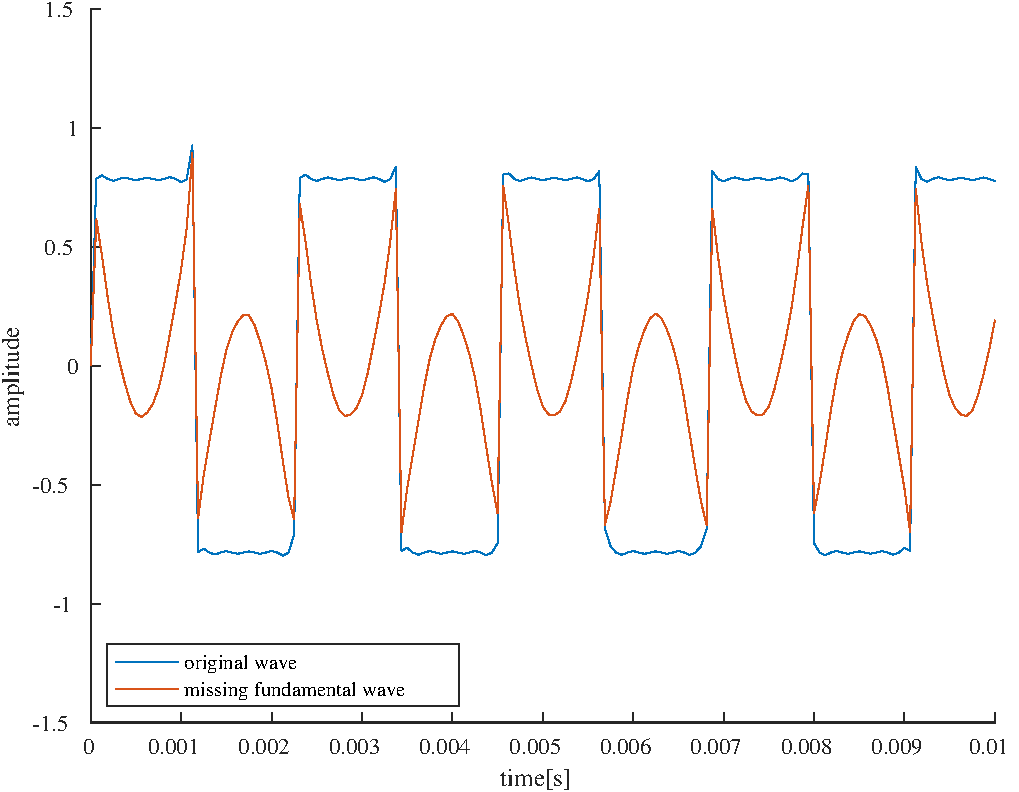
\includegraphics[keepaspectratio,width=\textwidth]{../../Figures/04_30_kukei.pdf}
        \subcaption{矩形波}
        \label{fig:ミッシングファンダメンタル_矩形波}
    \end{minipage}
    \begin{minipage}{.48\textwidth}
        \centering
        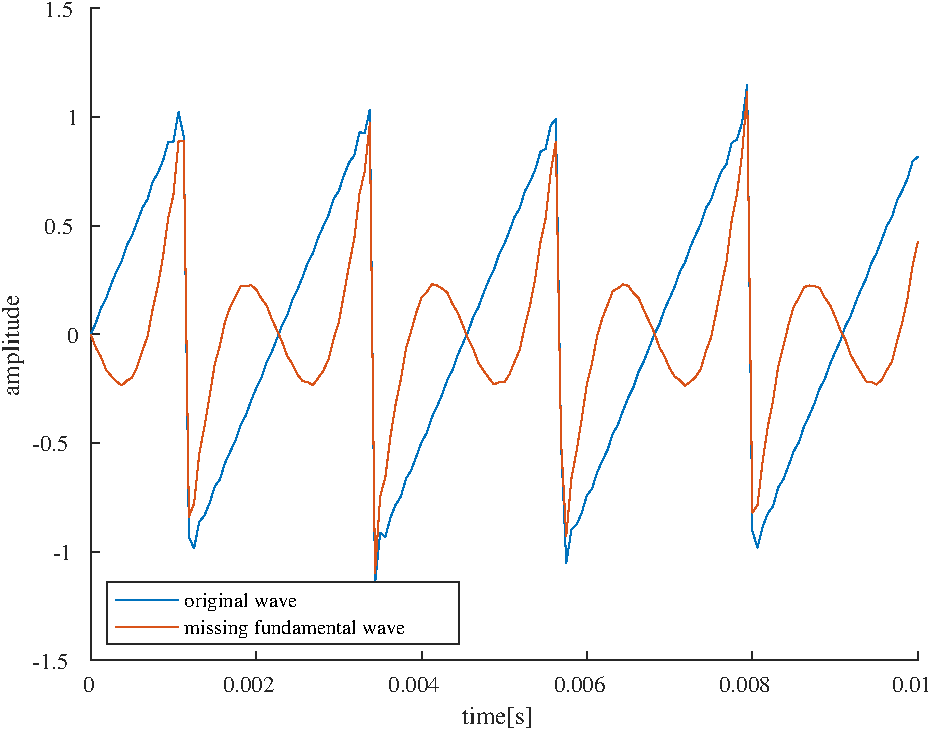
\includegraphics[keepaspectratio,width=\textwidth]{../../Figures/04_31_nokogiri.pdf}
        \subcaption{ノコギリ波}
        \label{fig:ミッシングファンダメンタル_ノコギリ波}
    \end{minipage}
    \caption{原波形とミッシングファンダメンタル波の比較}
    \label{fig:原波形と基本周波数を除去した波形}
\end{figure}
\consideration
ミッシングファンダメンタルを聞き取ることができる理由として考えられるのが,原波形とミッシングファンダメンタル波の周期が一致している点である.\figref{fig:ミッシングファンダメンタル_矩形波}より,原波形のひげの部分とミッシングファンダメンタル波の最大値が目視では一致している.また,\figref{fig:ミッシングファンダメンタル_ノコギリ波}の最大値と最小値の時刻も目視では一致している.
これらから基本周波数が知覚できるのではないだろうか.